
The choice of frameworks for development was mainly given by the
constituent, since the existing software was written in Ruby on Rails
with KnockoutJS and a MongoDB database. The main server-side language
was thus Ruby, and the client-side code was written in CoffeeScript.
CoffeeScript is a scripting language which compiles into Javascript.\\

For the choice of testing-related frameworks, we choose to look for
frequently used and active developed open source frameworks.
Technologies that are used by many people intuitively often has more
resources on how they are used, and also has the advantage of being more
likely to be recognized by future developers. Active development of used
frameworks is crucial, most importantly since they are likely to be
incompatible with future versions of other frameworks (such as Rails).
Another benefit is that new features and bug fixes are released.\\

The Ruby Toolbox website \footnote{\url{https://www.ruby-toolbox.com/}},
which uses information from the Github and RubyGems websites was
consulted in order to find frameworks with mentioned qualities.\\

\subsection{Ruby test frameworks}
RSpec, RSpec-mocks, Cucumber, Capybara, FactoryGirl, Timecop, site\_prism. (wip)


\subsection{Javascript test frameworks}

There exists a few different Javascript testing frameworks. We had
previously good experiences from working with
Jasmine\footnote{\url{http://jasmine.github.io/}}. We found that this
framework also seemed to be very popular and had a plenty of useful
documentation\footnote{It is worth to mention that the Jasmine
documentation is basically its own test suite with some additional
comments. This works incredibly good when the tests are well written.}.
Its syntax is inspired by RSpec, which also is an advantage since that
framework is used on the server side.\\

The Jasmine framework provides a way of writing tests, but a test runner
is also required in order to run the tests. Jasmine ships with a basic
test runner which was used initially. Due to several issues, we switched
to Karma\footnote{\url{http://karma-runner.github.io/}}.


\subsection{Test coverage}
\label{sec:coverage_frameworks}

There are multiple different ways of analyzing test coverage, and the
properties and conditions for each different kind of test coverage are
discoursed in \fref{sec:coverage}. However, we were unable to find any
test coverage tools for Ruby which analyzed anything else than statement
coverage, which is the weakest test coverage metric. Quite much effort
was spent on finding such tool, but without any success. Several
websites and Stack Overflow-answers indicates that no such tool exists
for Ruby at the time of this writing \cite{web:coverage_ruby19,
so:c1c2_coverage, so:c1_coverage, web:toolbox_code_metrics}. On one
hand, some of these sources are rather old and might be outdated, which
would indicate that such tool could have been created recently. On the
other hand would at least some of these sources probably been updated if
such tool became available.\\

We ended up using the
SimpleCov\footnote{\url{https://github.com/colszowka/simplecov}} tool
for Ruby test coverage metrics. At the time of this writing, it is the
most used Ruby tool for test coverage. It is also actively developed,
works with recent Ruby versions and RSpec versions, and produces pretty
and easy- to-read coverage reports in HTML (see
\fref{fig:simplecov_report}).\cite{web:toolbox_code_metrics}\\

\begin{figure}
\centering
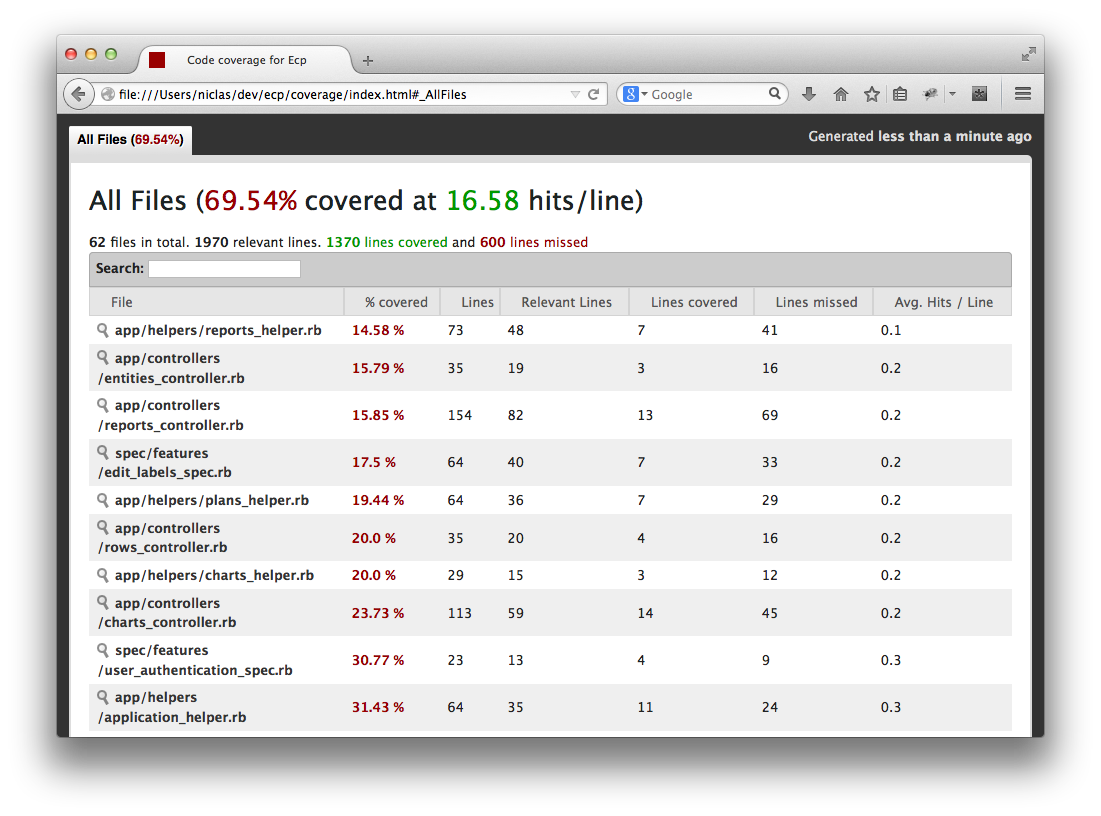
\includegraphics[width=1.0\textwidth]{methodology/simplecov}
\caption{A coverage report generated by SimpleCov}
\label{fig:simplecov_report}
\end{figure}

For the client-side CoffeeScript, we used a plug-in for the Karma test
runner called karma-coverage\footnote{\url{https://github.com/karma-
runner/karma-coverage}}. This tool basically integrates Karma with
Ibrik\footnote{\url{https://github.com/Constellation/ibrik}}, which is a
tool developed by Yahoo! for measuring test coverage of CoffeeScript
code. We did initially have some problems with getting this tool to work
correctly, since Ibrik internally uses another CoffeeScript compiler;
CoffeeScriptRedux, than the compiler used when tests itself are run.
CoffeeScriptRedux is more strict and yielded syntax errors in some of
our files, which could be compiled correctly in the production code. The
latest available release of Ibrik (version 1.1.1) also had major issues
with certain constructs in CoffeeScript, which made the files impossible
to analyze. This issues was however fixed in the development version.
Ibrik was first released in December 2013, which may explain its
immaturity. Ibrik internally uses istanbul-js for the coverage
analysis and report generation.\\

The chosen solution worked very well after sorting out the issues.
Statement coverage as well as branch coverage is supported, and it
yields useful reports. As with SimpleCov, the coverage reports are
produced as an interactive HTML report (see \fref{fig:karma_report}).\\

\begin{figure}
\centering
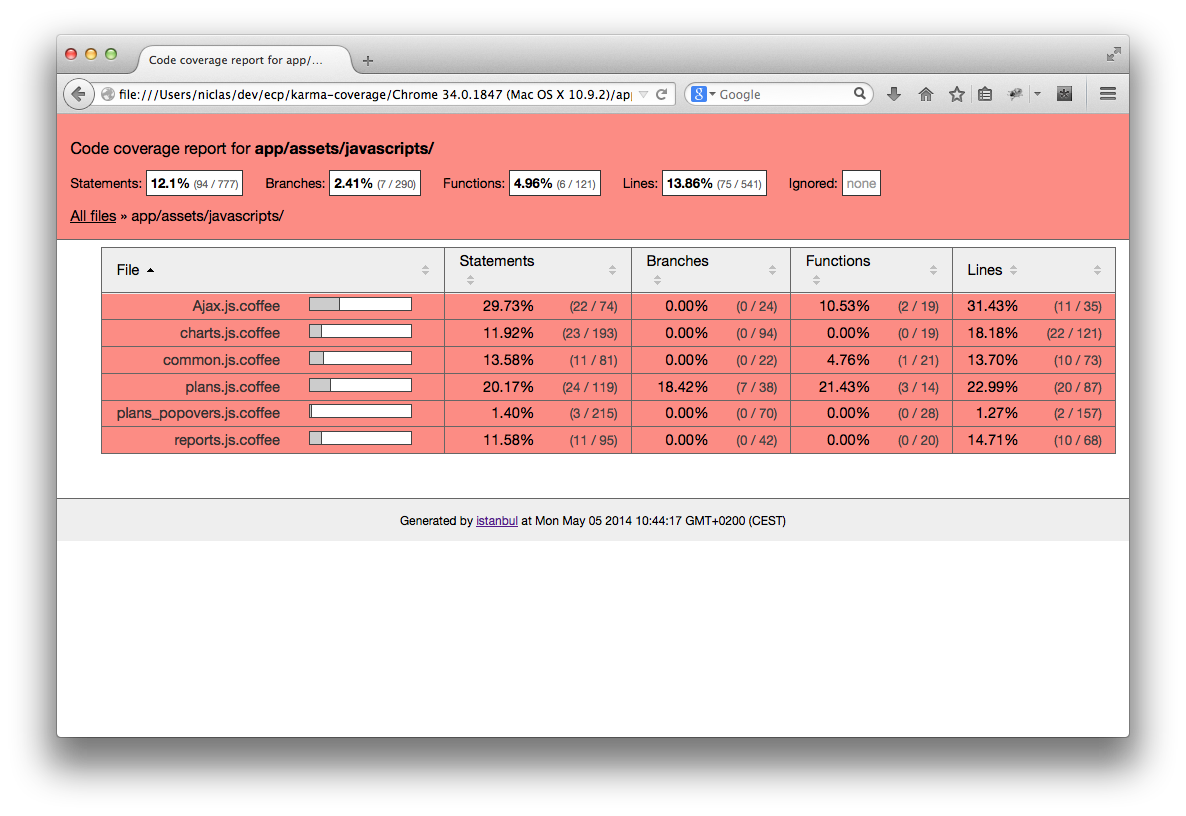
\includegraphics[width=1.0\textwidth]{methodology/karma_coverage}
\caption{A coverage report generated by istanbul-js using karma-coverage}
\label{fig:karma_report}
\end{figure}


\subsection{Mutation analysis}

There exists a few different tools for mutation analysis of Javascript
code. The ones we have found originates from academic research papers.
\citet{paper:mutandis} proposes a solution which has been implemented as
a tool called Mutandis
\footnote{\url{https://github.com/saltlab/mutandis/}}.
\citet{paper:ajaxmutator} presents another approach which has been
released as AjaxMutator \footnote{\url{https://github.com/knishiura-
lab/AjaxMutator}}. \citet{paper:webmujava} proposes a system-level
mutation testing approach called webMuJava.\\

Mutandis is based on website crawling tests. Although
\citeauthor{paper:mutandis} mentions that pure Javascript frameworks
have been tested using this tool, its implementation showed to be too
specific to be considered in our context. webMuJava does not seem to be
publicly available, and also seems to be too tightly integrated with a
specific back-end technique to be useful for Javascript-testing only.
